\documentclass[a0,landscape]{a0poster}
\usepackage{times}
\usepackage{graphicx}
\usepackage{multicol}
\usepackage{geometry}
\usepackage{qrcode}
\usepackage{amssymb}
\usepackage[most]{tcolorbox}
\usepackage{alltt}

% --- Page Geometry (Set to 48x36 inches with a 0.5-inch margin) ---
\geometry{papersize={48in,36in}, margin=0.5in}

% --- Custom Box Style ---
\newtcolorbox{posterbox}[1]{
    colback      = blue!5!white,
    colframe     = blue!75!black,
    fonttitle    = \bfseries\huge,
    title        = {#1},
    breakable,
    boxsep       = 8mm,
    arc          = 5mm,
}

\begin{document}
\pagestyle{empty}

% === TITLE BLOCK ===
\begin{center}
    \veryHuge \textbf{A Software Tool for Planning Better Clinical Trials} \\
    \vspace{0.25cm}
    \rule{\linewidth}{1.5pt}
    \vspace{0.25cm}
    \Huge Presenter: \textbf{Arnab Aich} \hspace{1cm} Mentor: \textbf{Yuan Zhang}\\
    \huge \textit{Department of Preventive Medicine, University of Tennessee Health Science Center}
\end{center}
\vspace{0.5cm}

% === FLEXIBLE 3-COLUMN LAYOUT ===
\begin{minipage}[t][\dimexpr\textheight-1cm\relax][t]{0.32\linewidth} % --- LEFT COLUMN ---

\begin{posterbox}{From Trial Setup to a Better Metric}
    \subsection*{\Large Basic Setup of a Clinical Trial}
    \Large
    In many studies, we compare two groups of patients:
    \begin{itemize} \itemsep=0.5em
        \item A \textbf{Treatment} group receiving a new medicine.
        \item A \textbf{Control} group receiving a placebo or standard care.
    \end{itemize}
    We then follow them over time to measure a **time-to-event** endpoint.

    \subsection*{\Large The Core Challenge: Study Design}
    \Large
    Before starting, researchers must answer two critical questions:
    \begin{enumerate} \itemsep=0.5em
        \item \textbf{Sample Size:} "How many patients do we need for a reliable result?"
        \item \textbf{Power:} "Given our patients, what is our chance of success?"
    \end{enumerate}
    
    \subsection*{\Large Why Traditional Methods Can Be Problematic}
    \Large
    Traditional metrics like the \textbf{Hazard Ratio (HR)} rely on strong assumptions that are often violated in the real world, making results hard to interpret.
    
    \subsection*{\Large A Better Metric: RMST}
    \Large
    Instead, we use \textbf{RMST} (Restricted Mean Survival Time). It directly measures the average "event-free" time patients experience.
    \begin{itemize} \itemsep=0.5em
        \item[\Large\checkmark]  It is easy for everyone to understand.
        \item[\Large\checkmark]  It provides a clear measure of treatment benefit.
    \end{itemize}
    
    \begin{center}
        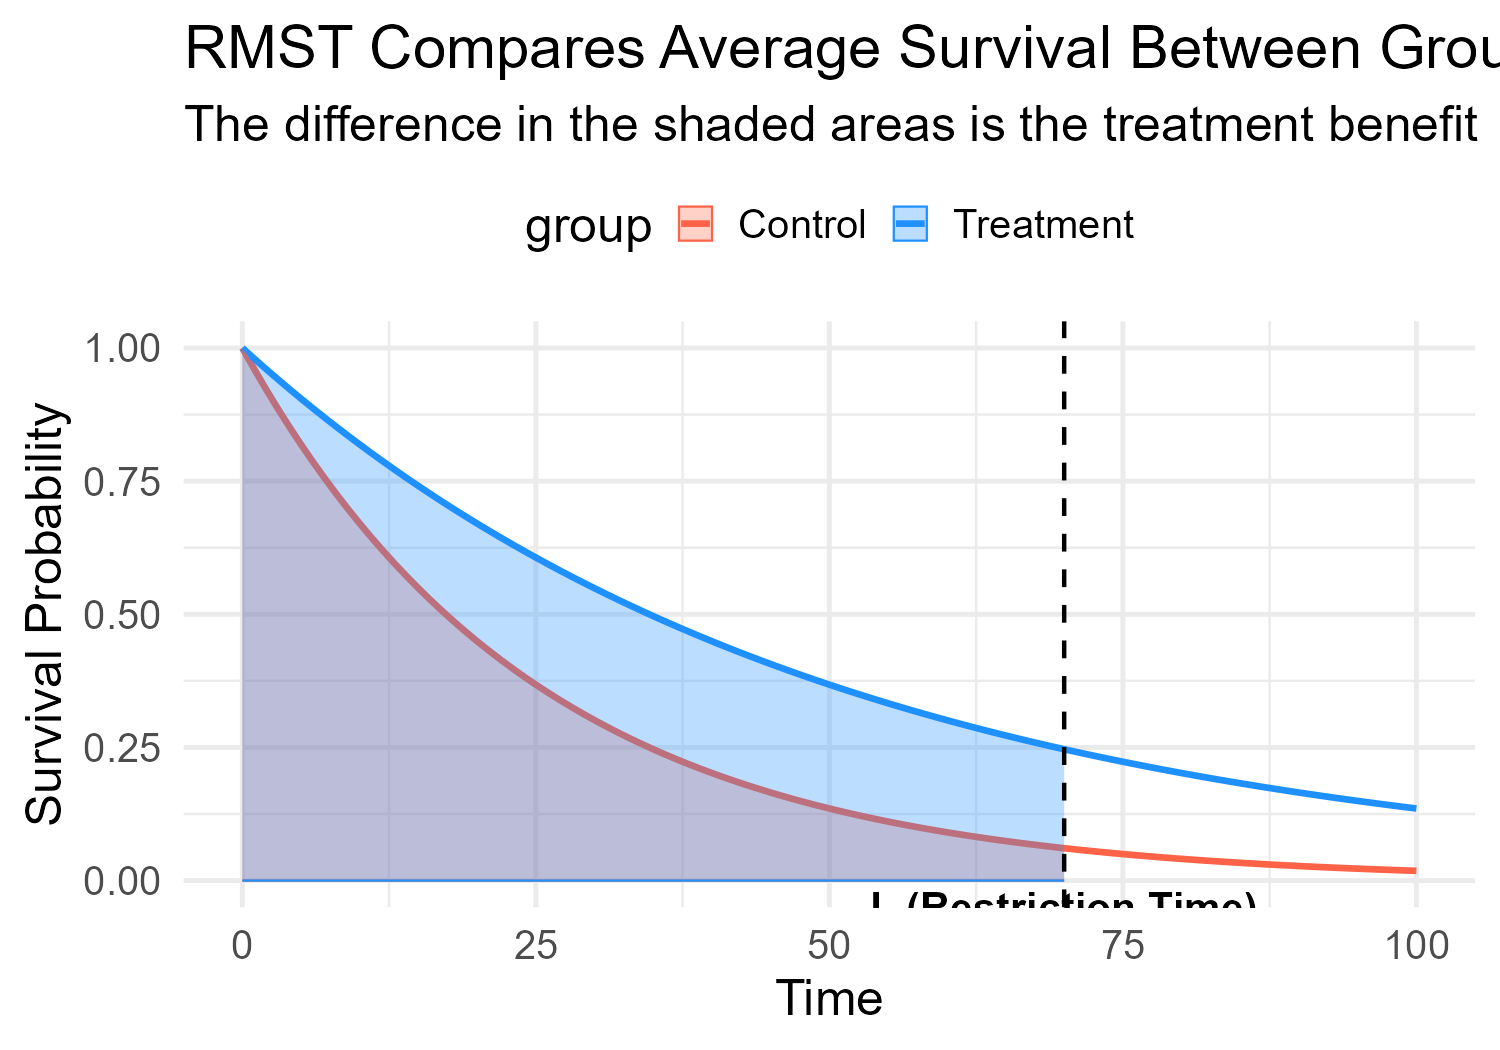
\includegraphics[width=0.9\linewidth]{rmst_causal_plot.png}
    \end{center}
\end{posterbox}

\end{minipage}
\hfill
\begin{minipage}[t][\dimexpr\textheight-1cm\relax][t]{0.34\linewidth} % --- CENTER COLUMN ---

\begin{posterbox}{Our Solution: The `RMSTSS` Tool}
    \Large
    Planning studies with RMST has been difficult. We made it easy. `RMSTSS` is a free tool that helps researchers properly plan modern medical studies.
    
    \begin{center}
        \vspace{0.5cm}
        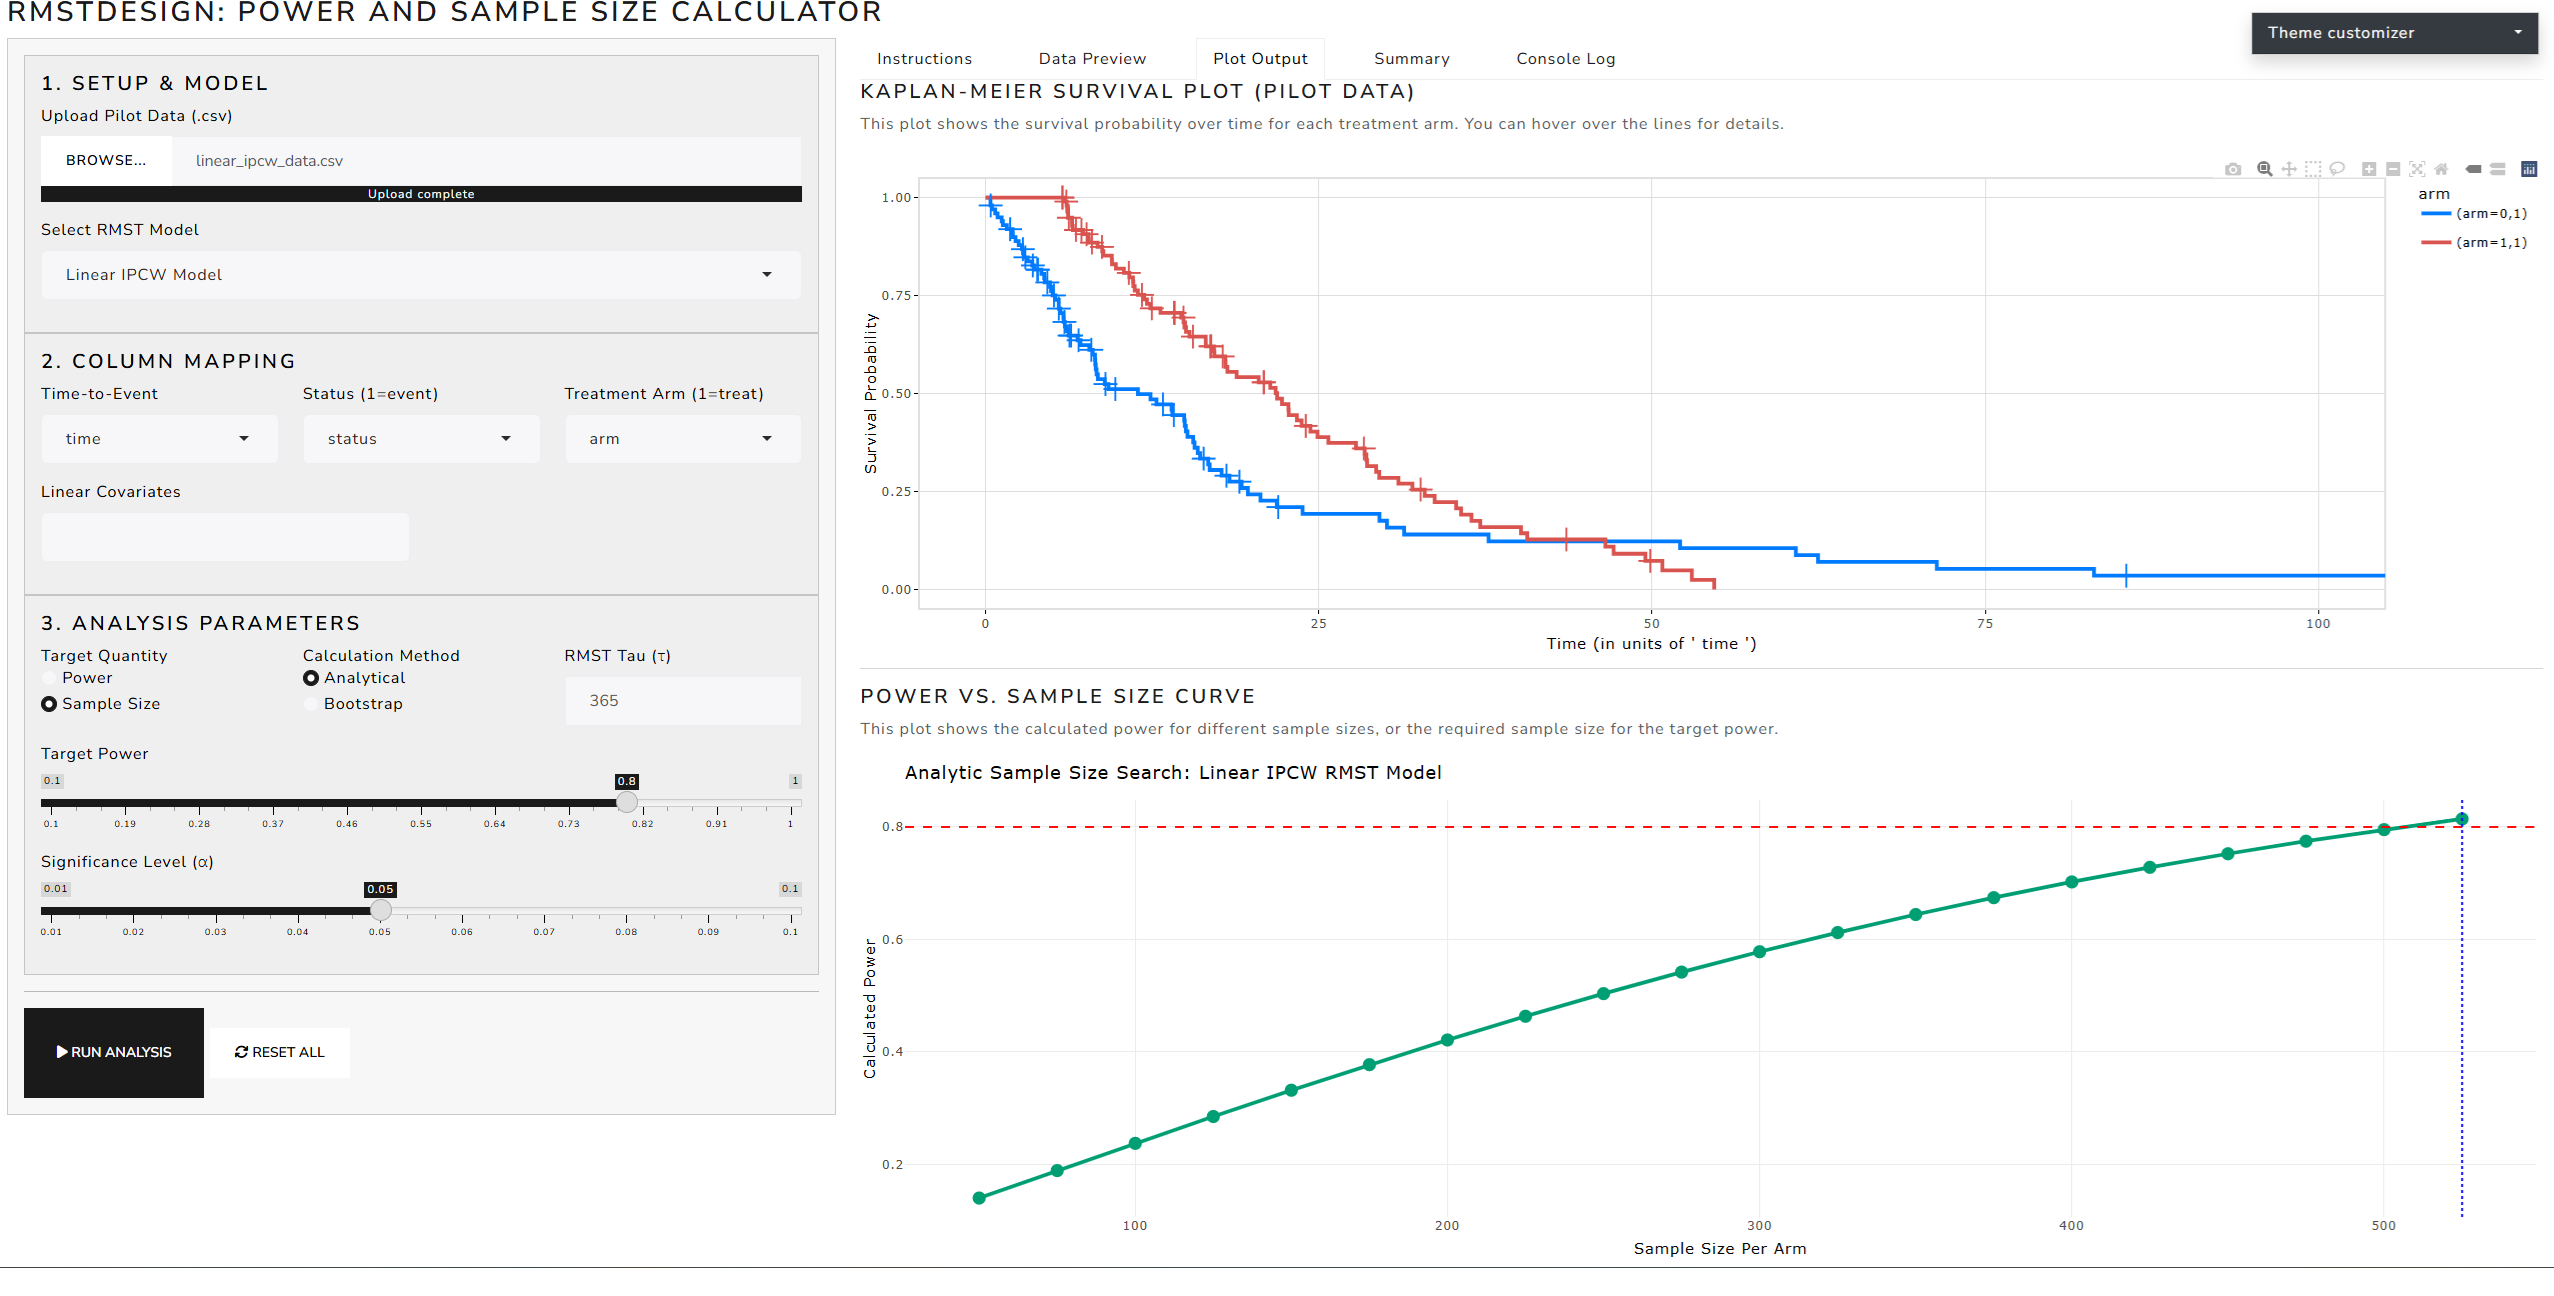
\includegraphics[width=0.9\linewidth]{app-ss.png}
        \vspace{0.5cm}
    \end{center}
    
    \subsection*{\Large How to Use the App}
    \Large
    The web application guides you through the process in a left-to-right flow:
    \begin{center}
        \Large
        \begin{tabular}{ccccccc}
            \textbf{Upload} & $\boldsymbol{\rightarrow}$ & \textbf{Choose Model} & $\boldsymbol{\rightarrow}$ & \textbf{Choose Goal} & $\boldsymbol{\rightarrow}$ & \textbf{Get Results!} \\
        \end{tabular}
    \end{center}

    \subsection*{\Large Features \& Capabilities}
    \begin{itemize} \itemsep=0.5em
        \item \Large \textbf{Multiple Models:} Handles standard trials, multi-hospital studies, and more.
        \item \Large \textbf{Clear Goals:} Calculate \textbf{Power} or search for the required \textbf{Sample Size}.
        \item \Large \textbf{Flexible Methods:} Use a \textbf{Quick Check} (Analytical) or a \textbf{Deep Dive} (Bootstrap).
    \end{itemize}
    
    \vfill 
    \begin{center}
        \qrcode[height=5cm]{https://arnab96.shinyapps.io/uthsc-app/}
    \end{center}
\end{posterbox}

\end{minipage}
\hfill 
\begin{minipage}[t][\dimexpr\textheight-1cm\relax][t]{0.32\linewidth} % --- RIGHT COLUMN ---

\begin{posterbox}{The `RMSTSS` R Package}
    \huge
    For statisticians and developers, `RMSTSS` is available as a powerful and flexible R package for use in scripts and analysis pipelines.
    
    \subsection*{\huge Key Functions \& When to Use Them}
    \Large
    The package provides a suite of functions for different trial designs:
    
    \vspace{0.5cm}
    \begin{tabular}{|p{0.35\linewidth}|p{0.55\linewidth}|}
        \hline
        \textbf{\Large Function Group} & \textbf{\Large Use Case} \\
        \hline
        \texttt{linear.*()} & Standard clinical trials. \\ \hline
        \texttt{additive.*()} & Multi-hospital trials (constant benefit). \\ \hline
        \texttt{MS.*()} & Multi-hospital trials (proportional benefit). \\ \hline
        \texttt{GAM.*()} & For complex, non-linear effects. \\ \hline
        \texttt{DC.*()} & Studies with competing outcomes. \\
        \hline
    \end{tabular}

    \subsection*{\huge Installation Guide}
    \Large
    Install the development version directly from GitHub:
    \begin{alltt}
remotes::install_github(
  "UTHSC-Zhang/RMSTSS-Package"
)
    \end{alltt}

    \vfill % Pushes content below to the bottom
    
    \subsection*{\huge Project Website}
    \begin{center}
        \qrcode[height=5cm]{https://github.com/UTHSC-Zhang/RMSTSS-Package}
    \end{center}

    \vspace{0.5cm}\hrule\vspace{0.5cm}
    
    \subsection*{\huge Key References}
    \small
    Royston \& Parmar (2013), Tian et al. (2014), Uno et al. (2014), Wang et al. (2018, 2019), Zhang \& Schaubel (2012).
\end{posterbox}

\end{minipage}

\end{document}